\documentclass[10pt,conference]{IEEEtran}
\IEEEoverridecommandlockouts
\usepackage[utf8]{inputenc}
\usepackage[T1]{fontenc}
\usepackage{microtype}
\usepackage{amsmath,amssymb}
\usepackage{amsthm}
\usepackage{graphicx}
\usepackage{hyperref}
\usepackage{booktabs}
\usepackage{multirow}
\usepackage{url}
\usepackage{algorithm}
\usepackage[table]{xcolor}
\usepackage{algpseudocode}
\usepackage{threeparttable}
\usepackage{cite}
\usepackage{subcaption}
\usepackage{tikz}
\usetikzlibrary{positioning, arrows.meta, calc, patterns}

\newtheorem{definition}{Definition}
\newcommand{\pend}{\textcolor{gray}{pend.}}   % result still running (see results/bench/PROGRESS.md)

\bibliographystyle{IEEEtran}

\title{Read Less, Answer Faster:\\In-Model Prompt Sieving for Long-Context Prefill and Decode}
\newif\ifanon\anontrue   % \anonfalse for the camera-ready version
\author{\ifanon\IEEEauthorblockN{Anonymous Authors}\else
    % TODO(authors): complete the author list and affiliations
    \IEEEauthorblockN{Quang Nguyen}
    \IEEEauthorblockA{
        \textit{Posts and Telecommunications Institute of Technology, Ha Noi, Vietnam} \\
        Email: nguyenquang71103@gmail.com
    }
\fi
}

\begin{document}

\maketitle
\bstctlcite{IEEEexample:BSTcontrol}

\begin{abstract}
Assistants that answer live from large document collections run without a reasoning phase, so their latency is set by prefilling a prompt of a hundred thousand tokens and decoding over its KV cache. Pruning the prompt with a small draft model fails where pruning matters most: the draft discards evidence it cannot find itself, and a 1.5B draft keeping half of the prompt loses 41\% of its 7B target's InfiniteBench score. Selecting tokens inside the target avoids this gap, but existing methods cut once and either cut too early (FastKV) or postpone the cut to stay accurate (ASL). We present \textbf{LayerSieve}, which keeps a prefix of layers dense, removes whole low-attention text units layer by layer down to a floor, and reuses the deep selection to shrink the shallow KV cache for decoding. On Qwen2.5-7B-Instruct-1M, LayerSieve matches dense and ASL accuracy on InfiniteBench and RULER, prefilling $1.24\times$ and decoding $1.27\times$ faster than ASL at 256k tokens and decoding $1.86\times$ faster than dense at 1M. Controlled single cuts show that accuracy at a given cost is decided by the depth where pruning ends, and a schedule defined in relative depth transfers without tuning across Qwen2.5 models from 3B to 32B.
\end{abstract}

\begin{IEEEkeywords}
Large Language Models, Long-Context Inference, Prompt Pruning, Token Pruning, KV Cache, Prefill Acceleration
\end{IEEEkeywords}

% =====================================================================
\section{Introduction}
\label{sec:intro}

Long-context inference has become a common regime of LLM applications rather than an edge case~\cite{bai2024longbench,ruler2024}. A typical deployment is an assistant that answers from a large body of documents while a person waits: Verizon, for example, fed nearly 15{,}000 internal documents into a Gemini model that answers the questions of its 28{,}000 customer-service agents on screen during live calls\footnote{Reuters, Apr.~9, 2025: \url{https://www.aol.com/news/verizon-says-google-ai-customer-120648406.html}}. Such an assistant gathers and summarizes facts from many retrieved passages rather than reasoning over them, so it can run without a reasoning phase and starts its answer right away. What remains is the cost of the context itself, in both stages: on an H200, Qwen2.5-7B-Instruct-1M takes 13.2\,s to prefill 128k tokens, and every answer token then reads the KV cache of all of them (Section~\ref{sec:exp-speed}). Whenever the prompt is new to the server---a new set of retrieved documents, a new repository, the first turn of a session---its prefill cannot be served from a prefix cache. Open models now accept these lengths~\cite{qwen25_1m}, but the cost of reading them does not shrink: prefill attention grows quadratically with the prompt and every decoding step reads a KV cache that grows linearly with it, even with IO-aware kernels and paged memory~\cite{dao2022flashattention,dao2024flashattention2,kwon2023efficient}.

The most direct way to cut both costs is to read fewer tokens. Prompt compression methods score tokens with an external model and send only the survivors to the target LLM~\cite{li2023selective,jiang2023llmlingua,jiang2024longllmlingua}; Speculative Prefill (SpecPrefill) makes this practical for serving by scoring with a small draft from the same family and reusing the target's positions~\cite{liu2025specprefill,upasani2026crossfamily}. The weakness of this design is structural: the scorer is weaker than the reader. Lookups of the kind above are where this matters, because the answer is one entry among many near-identical ones. Whenever the draft cannot locate the evidence itself---a key buried among thousands of near-identical UUID keys, the next hop of a variable chain---it ranks that evidence as unimportant and the target never sees it. We measure this directly in Section~\ref{sec:motivation}: on cases the 7B target solves, a 1.5B draft solves only 9 of 30 variable-tracking prompts, and SpecPrefill keeping 50\% of the prompt drops the target's InfiniteBench KV-retrieval accuracy from 66 to 34. Larger drafts or higher keep ratios shrink the gap but also the speedup.

The alternative is to let the target model choose. Its own attention at intermediate layers already concentrates on the tokens the answer depends on~\cite{li2024snapkv,shi2024gemfilter}, so tokens can be dropped from the forward pass after a few dense layers, removing both their prefill compute and their KV cache in deeper layers~\cite{fu2024lazyllm,long2026sliminfer}. Recent work makes this a single cut: FastKV propagates a fixed subset of tokens from one selection layer onward~\cite{jo2026fastkv}, and ASL picks that layer adaptively per input from the variance of token ranks~\cite{taniguchi2026asl}. A single cut must be both late enough to be accurate and early enough to be fast. We find that FastKV, cutting at layer 15 of 28, loses more than half of the multi-key needle accuracy on RULER at 32k, while ASL stays accurate by postponing the cut, mostly to layers 17--23, and not cutting at all on a quarter of RULER prompts, which leaves most of the prefill dense.

We propose \textbf{LayerSieve}, an in-model prompt pruning method that replaces the single cut with a sieve (Fig.~\ref{fig:teaser}). A dense prefix of layers, about 60\% of the depth, runs on the whole prompt; from the start layer $\ell_0$ on, every layer removes a fixed fraction of the remaining tokens, scored by the attention the last prompt tokens pay to them at that layer, until a floor fraction is reached. Removal happens at the granularity of text units (lines and clauses), so an identifier is either kept whole or dropped whole. Because each layer re-scores only survivors, a token wrongly kept at one layer can still be removed later, and the deep-layer selection is finally reused to shrink the KV cache of the dense shallow layers, so decoding also reads fewer tokens.

\begin{figure}[t]
\centering
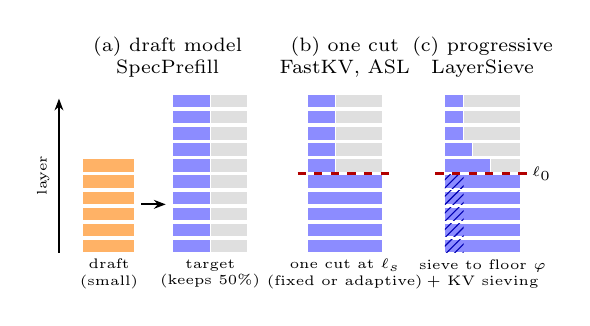
\begin{tikzpicture}[x=1.2cm,y=0.17cm,
  bar/.style={fill=blue!45,draw=white,line width=0.4pt},
  cut/.style={fill=gray!25,draw=white,line width=0.4pt},
  kv/.style={pattern=north east lines,pattern color=blue!70!black,draw=none}]
  % (a) draft-model pruning
  \foreach \i in {0,...,5} \fill[fill=orange!60,draw=white] (0,\i*1.2) rectangle (0.55,\i*1.2+1);
  \node[font=\tiny,align=center] at (0.28,-1.6) {draft\\(small)};
  \draw[-{Stealth[length=1.5mm]},thick] (0.62,3.6) -- (0.88,3.6);
  \foreach \i in {0,...,9} {\fill[cut] (0.95,\i*1.2) rectangle (1.75,\i*1.2+1); \fill[bar] (0.95,\i*1.2) rectangle (1.35,\i*1.2+1);}
  \node[font=\tiny,align=center] at (1.35,-1.6) {target\\(keeps 50\%)};
  \node[font=\scriptsize,align=center] at (0.9,14.6) {(a) draft model\\SpecPrefill};
  % (b) one-shot in-model
  \begin{scope}[xshift=2.85cm]
  \foreach \i in {0,...,9} \fill[cut] (0,\i*1.2) rectangle (0.8,\i*1.2+1);
  \foreach \i in {0,...,4} \fill[bar] (0,\i*1.2) rectangle (0.8,\i*1.2+1);
  \foreach \i in {5,...,9} \fill[bar] (0,\i*1.2) rectangle (0.3,\i*1.2+1);
  \draw[red!70!black,thick,dashed] (-0.1,5.9) -- (0.9,5.9);
  \node[font=\tiny,align=center] at (0.4,-1.6) {one cut at $\ell_s$\\(fixed or adaptive)};
  \node[font=\scriptsize,align=center] at (0.4,14.6) {(b) one cut\\FastKV, ASL};
  \end{scope}
  % (c) LayerSieve
  \begin{scope}[xshift=4.6cm]
  \foreach \i in {0,...,9} \fill[cut] (0,\i*1.2) rectangle (0.8,\i*1.2+1);
  \foreach \i in {0,...,4} {\fill[bar] (0,\i*1.2) rectangle (0.8,\i*1.2+1); \fill[kv] (0,\i*1.2) rectangle (0.2,\i*1.2+1);}
  \foreach \i/\w in {5/0.48,6/0.29,7/0.2,8/0.2,9/0.2} \fill[bar] (0,\i*1.2) rectangle (\w,\i*1.2+1);
  \draw[red!70!black,thick,dashed] (-0.1,5.9) -- (0.9,5.9);
  \node[font=\tiny,anchor=west] at (0.82,5.9) {$\ell_0$};
  \node[font=\tiny,align=center] at (0.4,-1.6) {sieve to floor $\varphi$\\+ KV sieving};
  \node[font=\scriptsize,align=center] at (0.4,14.6) {(c) progressive\\LayerSieve};
  \end{scope}
  \draw[-{Stealth[length=1.5mm]}] (-0.25,0) -- node[rotate=90,above,font=\tiny] {layer} (-0.25,11.5);
\end{tikzpicture}
\caption{Where the prompt is pruned. Each bar is one layer (bottom: first layer); its blue width is the fraction of prompt tokens the layer processes. (a) A small draft model scores tokens and the target reads only the survivors at every layer. (b) In-model one-shot selection runs the target densely up to layer $\ell_s$ and keeps a fixed subset afterwards. (c) LayerSieve runs a dense prefix, then removes a fraction of the surviving text units at every layer down to a floor; after prefill, the shallow layers keep only the KV of the final survivors (hatched) so decoding reads less cache.}
\label{fig:teaser}
\end{figure}

Our contributions are:
\begin{itemize}
  \item We show, on controlled hard cases and on InfiniteBench, that draft-model prompt pruning loses the evidence that the draft itself cannot find, and that this gap is invisible on easier needle-style benchmarks (Section~\ref{sec:motivation}).
  \item We propose LayerSieve, a progressive in-model pruning schedule with unit-level removal, a keep floor, and decode-time KV sieving, implemented in vLLM with CUDA-graph decoding (Section~\ref{sec:method}).
  \item We show that LayerSieve matches dense and ASL accuracy on InfiniteBench and RULER at 32k--128k while being faster than ASL in both prefill and decode, and that it outperforms SpecPrefill, SlimInfer and FastKV at matched compute; at equal cost, a single cut with our scorer and text units is as accurate only when it is placed where our schedule ends its descent (layers 17--18 of 28) and loses accuracy when placed earlier, so the end depth of pruning, not its gradualness, is what decides accuracy (Sections~\ref{sec:exp-main}--\ref{sec:exp-speed}, \ref{sec:ablation}).
  \item We show how to set the schedule for a new model: on Qwen2.5 from 3B to 32B, evidence becomes identifiable at half of the depth, the number of tokens kept at the last layer should be a fixed fraction of the prompt, and a schedule defined in relative depth preserves accuracy at the same cost for every size; KV sieving makes decoding $1.86\times$ faster at 1M tokens (Sections~\ref{sec:exp-speed}--\ref{sec:exp-start}).
\end{itemize}

% =====================================================================
\section{Related Work}
\label{sec:related}

\textbf{Prompt compression with an external scorer.}
Selective Context removed low self-information phrases using a small language model~\cite{li2023selective}, and LLMLingua and LongLLMLingua compressed prompts coarse-to-fine with a budget controller and question-aware perplexity from a small model~\cite{jiang2023llmlingua,jiang2024longllmlingua}. SpecPrefill transferred the idea of speculative decoding~\cite{leviathan2023speculative} to the prompt: a small draft from the same family ranked tokens by its attention, and the target prefilled only the top fraction at their original positions, giving large TTFT gains for 70B--405B targets~\cite{liu2025specprefill}; Cross-Family SpecPrefill relaxed the shared-tokenizer requirement~\cite{upasani2026crossfamily}. All of these methods bounded selection quality by the scorer, which was smaller than the reader.

\textbf{KV cache eviction for decoding.}
StreamingLLM kept attention sinks and a recent window~\cite{xiao2024efficient}, H2O kept heavy-hitter tokens~\cite{zhang2024h2o}, SnapKV selected the KV entries that an observation window at the end of the prompt attended to~\cite{li2024snapkv}, and PyramidInfer and PyramidKV shrank the retained cache with depth~\cite{yang2024pyramidinfer,cai2024pyramidkv}. ChunkKV and SepLLM kept or summarized contiguous chunks or segments instead of single tokens~\cite{liu2025chunkkv,chen2025sepllm}, the KV-cache analogue of our text units. Query-aware sparse attention instead loaded only relevant pages or blocks at each step~\cite{tang2024quest,xiao2024infllm}, and MInference and FlexPrefill applied dynamic sparse patterns to prefill attention~\cite{jiang2024minference,lai2025flexprefill}; these methods are orthogonal to ours, since they sparsify attention within a layer while LayerSieve removes tokens from all later projections and MLPs.

\textbf{In-model token pruning during prefill.}
LazyLLM pruned tokens progressively by the attention of the previous layer and allowed pruned tokens to be revived~\cite{fu2024lazyllm}. GemFilter selected tokens with the attention of an early layer and re-ran the full model on the selection~\cite{shi2024gemfilter}. SlimInfer removed hidden states block-wise at a few fixed layers~\cite{long2026sliminfer}. FastKV ran the full context up to a token-selective propagation layer and forwarded only the selected tokens beyond it, decoupled from the KV budget of earlier layers~\cite{jo2026fastkv}, and ASL chose that layer per input by monitoring the variance of attention-based token ranks~\cite{taniguchi2026asl}. These methods either cut early with a fixed schedule or cut once, so a selection made before the evidence was identifiable could not be corrected.

\textbf{Positioning.}
Table~\ref{tab:positioning} contrasts the families. LayerSieve selects with the target itself, refines its selection at every layer after a depth where evidence is reliably identifiable, removes whole text units, and carries the deep selection back to the shallow KV cache, so it reduces prefill compute and decoding cost together. Progressive pruning itself is not new: LazyLLM pruned from the first layers on and kept an auxiliary cache to revive tokens. Unit-level selection is not new either~\cite{liu2025chunkkv,chen2025sepllm}, and we give it to single-cut baselines in our ablation. What we add is \emph{where} pruning should start and \emph{where} it should end: we show that selection is unreliable before mid-depth in models from 3B to 32B, that at equal cost the depth where pruning ends decides accuracy more than whether removal is gradual, that this depth must scale with the model, and that a floor is needed for aggregation (Sections~\ref{sec:exp-start} and~\ref{sec:ablation}).

\begin{table}[t]
\centering
\caption{Positioning of LayerSieve. \emph{Target}: selection uses the target model's own attention. \emph{Start}: where token selection first acts. \emph{Refined}: the selection is revised after the first cut. \emph{Prefill}/\emph{Decode}: the method reduces that stage's cost.}
\label{tab:positioning}
\setlength{\tabcolsep}{3pt}
\small
\begin{tabular}{lccccc}
\toprule
Method & Target & Start & Refined & Prefill & Decode \\
\midrule
LLMLingua~\cite{jiang2023llmlingua} & -- & input & -- & \checkmark & \checkmark \\
SpecPrefill~\cite{liu2025specprefill} & -- & input & -- & \checkmark & \checkmark \\
SnapKV~\cite{li2024snapkv} & \checkmark & output & -- & -- & \checkmark \\
PyramidInfer~\cite{yang2024pyramidinfer} & \checkmark & early & -- & -- & \checkmark \\
LazyLLM~\cite{fu2024lazyllm} & \checkmark & early & stages & \checkmark & -- \\
SlimInfer~\cite{long2026sliminfer} & \checkmark & L8 & 3 steps & \checkmark & partial \\
FastKV~\cite{jo2026fastkv} & \checkmark & L15 & -- & \checkmark & partial \\
ASL~\cite{taniguchi2026asl} & \checkmark & adaptive & -- & \checkmark & partial \\
\textbf{LayerSieve} & \checkmark & $0.61L$ & every layer & \checkmark & \checkmark \\
\bottomrule
\end{tabular}
\end{table}

% =====================================================================
\section{Preliminaries}
\label{sec:prelim}

A decoder-only LLM with $L$ layers reads a prompt of $T$ tokens. Layer $\ell$ applies causal multi-head attention with $H$ query heads of dimension $d$ and rotary positions~\cite{su2024roformer}, followed by an MLP. During prefill every layer processes all $T$ tokens, so its cost is $O(T^2 d H)$ for attention plus $O(T)$ for projections and the MLP, and it stores $T$ key/value pairs; each decoding step then reads all $L\cdot T$ cached pairs. Time-to-first-token (TTFT) measures prefill latency and time-per-output-token (TPOT) measures decoding latency.

\begin{definition}[Draft-model prompt pruning~\cite{liu2025specprefill}]
A draft model $M_d$ scores every prompt token by its attention from the last prompt positions, a subset $S$ with $|S|=\kappa T$ is kept, and the target $M$ prefills only $S$ at its original positions in all $L$ layers.
\end{definition}

\begin{definition}[One-shot in-model selection~\cite{jo2026fastkv,taniguchi2026asl}]
The target runs layers $1,\dots,\ell_s-1$ on all tokens, scores them at layer $\ell_s$ by attention from an observation window, and layers $\ell_s,\dots,L$ process only the selected subset $S$, $|S|=\kappa T$. FastKV fixes $\ell_s$; ASL chooses $\ell_s$ per input once the rank variance of token scores falls below a threshold $\tau$, and does not cut if this never happens.
\end{definition}

\textbf{Measuring the budget.} Let $S_\ell$ be the set of tokens that layer $\ell$ actually processes: they form its queries and keys, pass through its MLP and are written to its KV cache. We compare methods by the token-layer fraction relative to dense, ignoring the scoring overhead:
\begin{equation}
C=\frac{1}{L}\sum_{\ell=1}^{L}\frac{|S_\ell|}{T}.
\label{eq:budget}
\end{equation}
$C$ is the average fraction of the prompt a layer processes, which sets the cost of projections and MLPs and, after prefill, the size of the KV cache. The \emph{budget} reported by FastKV and ASL, the number of tokens kept after the cut (e.g.\ 37.5\% or 2{,}048 tokens), does not determine $C$ by itself: the same keep ratio costs $C=\big(\ell_s-1+(L-\ell_s+1)\kappa\big)/L$, which depends on where the cut happens. We therefore match methods on $C$ rather than on their nominal keep ratio.

% =====================================================================
\section{Motivation and Observations}
\label{sec:motivation}

\subsection{A small draft model loses evidence it cannot find}
\label{sec:obs-draft}

We build a hard set of prompts up to 27k tokens on which the target Qwen2.5-7B-Instruct-1M is correct: synthetic key-value retrieval over UUID pairs in the style of InfiniteBench (kv)~\cite{zhang_etal_2024_bench}, variable tracking with distractor chains in the style of RULER (vt)~\cite{ruler2024}, and two-hop QA from HotpotQA and 2WikiMultihopQA as packaged by LongBench~\cite{yang2018hotpotqa,ho2020constructing,bai2024longbench}. Table~\ref{tab:draft} compares the target with its 1.5B and 0.5B siblings and with SpecPrefill using the 1.5B draft.

\begin{table}[t]
\centering
\caption{Hard cases solved by the 7B target: 30 prompts per task on which the target is correct (counts of prompts correct, H200). SpecPrefill uses the 1.5B draft; LayerSieve uses its default schedule and keeps 27\% of the prompt at the last layer.}
\label{tab:draft}
\setlength{\tabcolsep}{4pt}
\small
\begin{tabular}{lcccc}
\toprule
Model / method & kv & vt & hotpot & 2wiki \\
\midrule
Target 7B (dense) & 30 & 30 & 30 & 30 \\
Draft 1.5B (dense) & 23 & 9 & 24 & 17 \\
Draft 0.5B (dense) & 7 & 1 & 15 & 16 \\
\midrule
SpecPrefill~\cite{liu2025specprefill}, keep 90\% & 30 & 23 & 30 & 29 \\
SpecPrefill~\cite{liu2025specprefill}, keep 50\% & 21 & 19 & 28 & 27 \\
SpecPrefill~\cite{liu2025specprefill}, keep 30\% & 9 & 19 & 30 & 24 \\
SpecPrefill~\cite{liu2025specprefill}, keep 10\% & 1 & 12 & 27 & 23 \\
LayerSieve, token-level & 14 & 29 & 30 & 28 \\
\textbf{LayerSieve}, unit-level & \textbf{30} & \textbf{30} & \textbf{30} & \textbf{29} \\
\bottomrule
\end{tabular}
\end{table}

The drafts fail most on exactly the tasks whose evidence is lexically indistinguishable from the distractors: the 1.5B draft solves 9 of 30 variable-tracking prompts and the 0.5B draft 1 of 30. SpecPrefill inherits this blindness. Keeping 30\% of the prompt, it loses more than two thirds of the kv prompts even though the target could answer all of them, and even at 90\% it loses 7 vt prompts, while the less demanding QA tasks are barely affected. The same pattern appears at 128k tokens in Section~\ref{sec:exp-main}: SpecPrefill keeping 50\% matches dense on RULER, whose needles are lexically salient, but loses 41\% of the dense InfiniteBench score, including half of the KV-retrieval accuracy. A benchmark of salient needles therefore overstates how safe draft-based pruning is.

\subsection{Evidence becomes identifiable only from mid-depth}
\label{sec:obs-depth}

If the target's own attention is the better scorer, the question is from which layer it can be trusted. We probe Qwen2.5 models of six sizes and variants with the kv and vt prompts, whose evidence spans are known: at every layer $\ell$ we score the prompt with the attention of the last 128 tokens, keep the top 25\% of text units, and measure the fraction of evidence kept. Fig.~\ref{fig:start}(b) plots the worst recall over all layers from $\ell$ on. Before roughly half of the depth, every model has layers at which a one-shot selection would discard 30--40\% of the evidence; recall becomes reliably complete only after $\ell/L\approx 0.5$ (0.5--0.6 for the 3B and 32B models). This agrees with the observation that intermediate layers carry the most task-relevant representations~\cite{skean2025layerbylayer}, and it implies two requirements: pruning should not start before mid-depth, and a selection made near that boundary should remain revisable by later, more reliable layers.

% =====================================================================
\section{Methodology}
\label{sec:method}

LayerSieve modifies the prefill forward pass of the target model and the layout of its KV cache; it adds no parameters and needs no draft model. Algorithm~\ref{alg:layersieve} in Appendix~\ref{app:impl} summarizes it.

\subsection{Scoring with the target's own attention}

Let $S_{\ell-1}$ be the tokens that survive into layer $\ell$; each keeps its original position for the rotary embedding. Two sets are never removed: the first 128 tokens, which act as attention sinks~\cite{xiao2024efficient}, and the last 128 tokens $O$, which hold the question and serve as the observation window, as in SnapKV~\cite{li2024snapkv}. Before a pruned layer runs, we compute its queries and keys for the survivors and let $a^{h}_{ij}$ be the causal attention weight from observation token $i\in O$ to survivor $j$ in head $h$. The score of token $j$ takes its strongest head and sums over the window,
\begin{equation}
s_j=\sum_{i\in O}\max_{h} a^{h}_{ij},
\label{eq:score}
\end{equation}
so a token that one retrieval head attends to is not diluted by heads that ignore it. Scoring is one attention of 128 queries over the survivors, small next to the layer itself.

\subsection{Removing whole text units}

Token-level selection keeps fragments: an identifier split across tokens may lose a few of them, which is enough to make a retrieved UUID wrong (Table~\ref{tab:draft}, kv). LayerSieve therefore partitions the prompt into units $u$ that end at a newline or at one of \texttt{. , ; ! ?}, with at most 128 tokens per unit, and scores each unit by its strongest token, $\hat s_u=\max_{j\in u}s_j$ with $s_j$ from Eq.~\eqref{eq:score}. Pruning removes the lowest-scoring units whole, so the kept prompt consists of complete lines and clauses.

\subsection{Progressive schedule with a floor}

We describe the schedule by the fraction $\kappa_\ell$ of the prompt that layer $\ell$ processes (sinks and observation window are always kept and not counted). The first $\ell_0$ layers are dense; after them, every layer keeps a fraction $1-\rho$ of what the previous layer kept, until a floor $\varphi$ is reached:
\begin{equation}
\kappa_\ell=\begin{cases}1, & \ell\le\ell_0,\\ \max\big((1-\rho)^{\ell-\ell_0},\ \varphi\big), & \ell>\ell_0.\end{cases}
\label{eq:sched}
\end{equation}
Before a layer $\ell>\ell_0$ runs, LayerSieve scores the survivors with that layer's attention (Eq.~\eqref{eq:score}) and removes the lowest-scoring units until $\kappa_\ell T$ tokens remain. Removed tokens leave the attention and MLP of all later layers. Since $\kappa_\ell=|S_\ell|/T$, the cost of Eq.~\eqref{eq:budget} is simply $C=\frac{1}{L}\sum_\ell\kappa_\ell$.

Each parameter has one role. The start $\ell_0$ delays pruning until attention identifies the evidence (Section~\ref{sec:obs-depth}). The rate $\rho$ makes selection progressive: every layer re-ranks only the survivors with its own attention, so a unit that looked relevant at one layer can still be removed by a deeper, more reliable one. The floor $\varphi$ protects aggregation tasks, such as counting frequent words, which need many occurrences rather than one needle; without it the prompt would shrink to $(1-\rho)^{L-\ell_0}$, 4\% for $\rho=0.25$ on 28 layers.

Our default for the 28-layer model is $\ell_0=17$, $\rho=0.4$, $\varphi=0.25$: 17 dense layers, then layers that keep 60\%, 36\% and, from the third pruned layer on, 25\% of the prompt, for $C=0.72$. Section~\ref{sec:exp-start} shows how to carry these values to models of other depths.

\subsection{KV sieving for decoding}

After prefill, layer $\ell$ holds the KV of $S_\ell$. The pruned layers already hold a small cache, but the dense prefix holds all $T$ entries, so decoding would still read the whole prompt at every step. With KV sieving at a reference layer $r$, every layer before $r$ keeps only the KV entries of $S_r$, the tokens that survived to layer $r$. This reuses the deep, reliable selection to compress the shallow layers, whose own attention is less selective. With the default schedule and $r=22$, the KV cache shrinks from 72\% to 25\% of dense. KV sieving does not change the first generated token, which is computed during prefill; it only affects later tokens.


\subsection{Implementation}

We implement LayerSieve as a patch of the model forward pass in vLLM 0.6.3~\cite{kwon2023efficient}\footnote{\url{https://github.com/vllm-project/vllm}}, with CUDA-graph decoding (details in Appendix~\ref{app:impl}). All LayerSieve timings include its scoring.

% =====================================================================
\section{Experiments and Results}
\label{sec:exp}

\subsection{Setup}
\label{sec:setup}

\textbf{Models and hardware.} The main model is Qwen2.5-7B-Instruct-1M ($L=28$)~\cite{qwen25_1m}\footnote{\url{https://huggingface.co/Qwen/Qwen2.5-7B-Instruct-1M}}; the start-layer study adds Qwen2.5-Instruct 3B, 7B, 14B, 32B and Qwen2.5-14B-Instruct-1M~\cite{qwen252024}. All measurements use one NVIDIA H200, greedy decoding and a batch of one request.

\textbf{Benchmarks.} InfiniteBench~\cite{zhang_etal_2024_bench}\footnote{\url{https://github.com/OpenBMB/InfiniteBench}}: Math.Find, Code.Debug, En.Dia and Retr.KV, 100 examples each sampled with seed 42, truncated to 128k tokens in the middle following the ASL evaluation protocol~\cite{taniguchi2026asl}. RULER~\cite{ruler2024}\footnote{\url{https://github.com/NVIDIA/RULER}}: all 13 tasks at 32k, 64k and 128k tokens, 100 examples per task and length sampled with seed 42 from 500 generated examples, scored by RULER's string-match metrics.

\textbf{Baselines.} SpecPrefill~\cite{liu2025specprefill} with a Qwen2.5-1.5B-Instruct draft, SlimInfer~\cite{long2026sliminfer}, FastKV~\cite{jo2026fastkv} and ASL~\cite{taniguchi2026asl}, each configured to the cost of LayerSieve ($C\approx0.72$) except ASL, whose adaptive cut leads to $C=0.84$--$0.89$. FastKV, ASL and SpecPrefill run their official code. Appendix~\ref{app:baselines} gives the configurations and how their cost is computed.

\textbf{LayerSieve.} $\ell_0=17$, $\rho=0.4$, $\varphi=0.25$, unit-level removal, with KV sieving at $r=22$ (LayerSieve) and without it (LayerSieve$_{\text{prefill}}$).

\subsection{Accuracy at matched cost}
\label{sec:exp-main}

\begin{table*}[t]
\centering
\caption{Accuracy on InfiniteBench (128k) and RULER on Qwen2.5-7B-Instruct-1M. All methods except ASL run at $C\approx0.72$; ASL's adaptive cut costs more. $C$: token-layer fraction relative to dense (Eq.~\eqref{eq:budget}); SpecPrefill includes its draft; ASL is measured from its realized cut layers (InfiniteBench / RULER). Bold: best pruning method per column. ASL at larger thresholds $\tau$, and methods that also compress the KV cache (SnapKV after a dense prefill, $C=1$), are evaluated on RULER at 128k only (--).}
\label{tab:main}
\setlength{\tabcolsep}{4.5pt}
\small
\begin{tabular}{l c ccccc cccc}
\toprule
& & \multicolumn{5}{c}{InfiniteBench} & \multicolumn{4}{c}{RULER} \\
\cmidrule(lr){3-7}\cmidrule(lr){8-11}
Method & $C$ & Math & Code & Dia & KV & Avg & 32k & 64k & 128k & Avg \\
\midrule
Dense & 1.00 & 37.0 & 22.0 & 11.0 & 66.0 & 34.0 & 89.7 & 85.8 & 83.7 & 86.4 \\
\midrule
SpecPrefill~\cite{liu2025specprefill} & 0.70 & 22.0 & 20.0 & 5.0 & 34.0 & 20.2 & 89.5 & 86.6 & 83.7 & 86.6 \\
SlimInfer~\cite{long2026sliminfer} & 0.74 & 37.0 & 21.0 & 10.0 & 42.0 & 27.5 & 82.2 & 80.1 & 76.9 & 79.7 \\
FastKV~\cite{jo2026fastkv} & 0.71 & 36.0 & 21.0 & 13.0 & 48.0 & 29.5 & 80.5 & 79.5 & 77.5 & 79.2 \\
ASL~\cite{taniguchi2026asl} & .84/.87 & 36.0 & 22.0 & 8.0 & 66.0 & 33.0 & \textbf{89.9} & \textbf{87.4} & 83.9 & \textbf{87.1} \\
ASL~\cite{taniguchi2026asl}, $\tau=0.45$ & .80/.81 & 36.0 & 21.0 & 9.0 & 64.0 & 32.5 & -- & -- & 83.4 & -- \\
ASL~\cite{taniguchi2026asl}, $\tau=0.6$ & .77/.77 & 37.0 & 21.0 & 11.0 & 62.0 & 32.8 & -- & -- & 81.9 & -- \\
\midrule
FastKV~\cite{jo2026fastkv} + KV compr. & 0.71 & 36.0 & 21.0 & \textbf{15.0} & 45.0 & 29.2 & -- & -- & 76.7 & -- \\
SnapKV~\cite{li2024snapkv}, KV 25\% & 1.00 & \textbf{38.0} & 22.0 & 11.0 & 43.0 & 28.5 & -- & -- & 78.6 & -- \\
\midrule
LayerSieve$_{\text{prefill}}$ & 0.72 & 35.0 & 21.0 & 11.0 & \textbf{67.0} & \textbf{33.5} & 88.9 & 86.7 & 83.9 & 86.5 \\
LayerSieve & 0.72 & 34.0 & \textbf{24.0} & 9.0 & 66.0 & 33.2 & 89.4 & 87.0 & \textbf{84.0} & 86.8 \\
\bottomrule
\end{tabular}
\end{table*}

Table~\ref{tab:main} reports the main comparison, and Table~\ref{tab:ruler128} RULER per task at 128k. The methods fall into three groups.

\textbf{Draft-model pruning fails where the draft is weak.} SpecPrefill matches dense on RULER, whose needles are lexically salient, but loses 41\% of the InfiniteBench score, including half of the KV-retrieval accuracy. This confirms Section~\ref{sec:obs-draft} at 128k tokens. The loss is not caused by extending the 1.5B draft beyond its native 32k window: on the same InfiniteBench examples truncated to 32k, SpecPrefill keeping 50\% scores 12.0 against 21.0 for dense and 20.8 for LayerSieve ($p<0.001$).

\textbf{Early single cuts lose multi-key retrieval.} SlimInfer and FastKV lose 6--9 RULER points at every length, mostly on the two hardest multi-key tasks, where FastKV scores 68 and 41 at 128k against 98 and 83 for dense. Their cut at layer 15 or earlier comes before the depth at which evidence becomes identifiable (Fig.~\ref{fig:start}b).

\textbf{LayerSieve matches ASL at a lower cost.} Both stay at the dense level, but LayerSieve costs $C=0.72$ against 0.84--0.87 for ASL, and with KV sieving keeps 25\% of the KV cache against 84--87\%. A paired bootstrap over examples (10{,}000 resamples) finds no significant difference between LayerSieve, ASL and dense on either benchmark ($p\ge0.06$), and significant gains over SlimInfer and FastKV on both and over SpecPrefill on InfiniteBench ($p<0.02$). The small RULER gap to ASL arises at 32k and 64k and comes from the common-word task (cwe) alone, where ASL exceeds dense at these lengths, possibly because removing distractor words eases counting; without cwe, the two are equal over all lengths (90.2 vs.\ 90.1).

\textbf{ASL cannot buy speed with its threshold.} A larger threshold $\tau$ makes ASL cut earlier. At $\tau=0.6$ its cost is still above LayerSieve's ($C=0.77$), yet it loses 2.0 RULER points at 128k ($p<0.001$), almost all on the hardest multi-key task. Cutting earlier costs ASL accuracy the same way it costs FastKV.

\textbf{KV compression does not replace prefill pruning.} SnapKV~\cite{li2024snapkv} keeps 25\% of the KV cache, as LayerSieve does with KV sieving, but after a dense prefill. It loses about 5 points on both benchmarks against LayerSieve$_{\text{prefill}}$ ($p\le0.004$), mostly on KV retrieval and multi-key needles. Adding the same compression before FastKV's cut lowers FastKV further.

\subsection{Prefill and decode speed}
\label{sec:exp-speed}

Speed depends only on which tokens each layer processes and caches, so we compare schedules in one engine. We run every schedule in our vLLM implementation with CUDA-graph decoding: FastKV as a single cut at layer 15 keeping 37.5\%, and ASL as single cuts at layers 17--23 weighted by the distribution of cut layers ASL actually chose on RULER 128k, with dense for the prompts it did not cut. This favors ASL, since its per-layer rank monitoring between layers 10 and the cut is not charged. Table~\ref{tab:speed} reports speedups over dense on two prompts per length.

\begin{table}[t]
\centering
\caption{Speedup over dense on Qwen2.5-7B-Instruct-1M (H200, CUDA-graph decoding, 256 output tokens). Dense TTFT is 13.2\,s / 48.6\,s and TPOT 9.3\,ms / 11.0\,ms at 128k / 256k. FastKV cuts at layer 15 keeping 37.5\%; ASL follows its realized cut layers, without its monitoring cost; SpecPrefill includes the draft's prefill. Rows below the line come from a second run (Appendix~\ref{app:baselines}).}
\label{tab:speed}
\setlength{\tabcolsep}{4pt}
\small
\begin{tabular}{lcccc}
\toprule
& \multicolumn{2}{c}{TTFT} & \multicolumn{2}{c}{TPOT} \\
\cmidrule(lr){2-3}\cmidrule(lr){4-5}
Schedule & 128k & 256k & 128k & 256k \\
\midrule
FastKV~\cite{jo2026fastkv} & \textbf{1.60$\times$} & \textbf{1.64$\times$} & 1.17$\times$ & 1.14$\times$ \\
ASL~\cite{taniguchi2026asl} & 1.22$\times$ & 1.23$\times$ & 1.08$\times$ & 1.06$\times$ \\
LayerSieve$_{\text{prefill}}$ & 1.49$\times$ & 1.53$\times$ & 1.08$\times$ & 1.09$\times$ \\
LayerSieve & 1.49$\times$ & 1.52$\times$ & \textbf{1.26$\times$} & \textbf{1.35$\times$} \\
\midrule
FastKV~\cite{jo2026fastkv} + KV compr. & 1.59$\times$ & \textbf{1.64$\times$} & 1.11$\times$ & 1.22$\times$ \\
SlimInfer~\cite{long2026sliminfer} & 1.59$\times$ & \textbf{1.64$\times$} & 1.03$\times$ & 1.14$\times$ \\
SpecPrefill~\cite{liu2025specprefill} & 1.45$\times$ & -- & 1.13$\times$ & -- \\
\bottomrule
\end{tabular}
\end{table}

At equal accuracy, LayerSieve prefills $1.22\times$ faster than ASL at 128k and $1.24\times$ at 256k, because ASL must postpone its cut, mostly to layers 17--23, or skip it to remain accurate, whereas LayerSieve starts at layer 17 and removes 40\% of the survivors per layer. With KV sieving, LayerSieve also decodes $1.17\times$ and $1.27\times$ faster than ASL, which keeps the full cache in all layers before its cut. FastKV and SlimInfer prefill fastest because their cuts come earlier, but at a 7-point RULER deficit (Table~\ref{tab:main}); compressing FastKV's pre-cut KV cache speeds up its decoding less than KV sieving does for LayerSieve at 256k (1.22$\times$ vs.\ 1.35$\times$) and costs further accuracy. SpecPrefill's draft prefill alone takes 39\% of the dense time at 128k, which bounds its speedup.

\begin{figure*}[t]
\centering
\includegraphics[width=\textwidth]{figures/pareto.pdf}
\caption{Accuracy versus prefill speedup at 128k on Qwen2.5-7B-Instruct-1M. Circles: LayerSieve variants ($\rho\in\{0.12,0.25,0.4\}$, with and without floor); star: default. The one-cut points use our scoring at FastKV's schedule (Table~\ref{tab:ablation}). ASL's speedup follows the cut layers it chose on each benchmark. Dotted: dense.}
\label{fig:pareto}
\end{figure*}

\textbf{The speed gap to ASL is structural.} One may ask whether ASL would match LayerSieve's speed with a smaller keep ratio. At its default threshold it cannot: ASL's cost is set by \emph{when} it cuts, not by how much it keeps. With its realized cut layers (median layer 20, no cut on 12\% of InfiniteBench and 25\% of RULER prompts), even keeping \emph{zero} tokens after the cut would cost $C=0.75$ on InfiniteBench and $0.79$ on RULER, more than LayerSieve's $C=0.72$ at dense accuracy. A larger threshold moves the cut earlier, which is what FastKV does, and Fig.~\ref{fig:pareto} shows the price: every single cut at layer 15, whether from FastKV or from our own scorer with units, loses accuracy, while LayerSieve variants between $1.33\times$ and $1.49\times$ all stay at the dense level on both benchmarks.

\subsection{Decoding up to 1M tokens}
\label{sec:exp-decode}

\begin{table}[t]
\centering
\caption{Decoding speedup (TPOT) over dense on Qwen2.5-7B-Instruct-1M up to 1M tokens (CUDA graph, 512 output tokens), with accuracy on the hard set (/120). Dense TPOT is 8.4\,ms at 128k and 23.8\,ms at 1M. The last two rows use no floor.}
\label{tab:decode}
\setlength{\tabcolsep}{3pt}
\small
\begin{tabular}{lccccc}
\toprule
Schedule & Hard & 128k & 256k & 512k & 1M \\
\midrule
Dense & 120 & 1.00$\times$ & 1.00$\times$ & 1.00$\times$ & 1.00$\times$ \\
LayerSieve$_{\text{prefill}}$ & 119 & 1.03$\times$ & 1.11$\times$ & 1.12$\times$ & 1.29$\times$ \\
LayerSieve ($r=22$) & 119 & 1.20$\times$ & 1.27$\times$ & 1.64$\times$ & \textbf{1.86$\times$} \\
\midrule
$\rho=0.25$ & 118 & 1.16$\times$ & 1.15$\times$ & 1.14$\times$ & 1.26$\times$ \\
$\rho=0.25$, $r=22$ & 117 & 1.27$\times$ & 1.54$\times$ & 1.70$\times$ & 2.17$\times$ \\
\bottomrule
\end{tabular}
\end{table}

For a long answer over a long document, decoding rather than prefill dominates the latency. Table~\ref{tab:decode} shows that prefill pruning alone barely accelerates decoding, because the dense prefix still holds the whole prompt in its KV cache. KV sieving removes that cache, and its gain grows with context length because KV reads take a growing share of each decoding step: with the default schedule, decoding becomes $1.20\times$ faster at 128k and $1.86\times$ at 1M tokens, without losing any hard-set prompt relative to LayerSieve$_{\text{prefill}}$, and prefill stays $1.55\times$ faster at 1M. A schedule without a floor reaches $2.17\times$ at 1M, but loses aggregation accuracy (Section~\ref{sec:ablation}), so we do not use it. The reference layer $r$ follows the same relative rule, $r\approx0.8L$; on the 14B-1M model ($r=38$) decoding becomes $1.66\times$ faster at 256k with KV sieving, against $1.20\times$ without it.

\subsection{Setting the schedule for a new model}
\label{sec:exp-start}

A new model needs values for $\ell_0$, $\rho$ and $\varphi$. We study six Qwen2.5 models from 3B (36 layers) to 32B (64 layers) on the hard set of Section~\ref{sec:obs-draft} and on three RULER 32k tasks that stress the schedule: multi-key retrieval (mk3) and the aggregation tasks cwe and fwe. Three questions arise.

\begin{figure*}[t]
\centering
\includegraphics[width=\textwidth]{figures/start_layer.pdf}
\caption{Start layer across Qwen2.5 models. (a) Accuracy on the hard set (percentage of dense-correct prompts kept) when sieving starts at relative depth $\ell_0/L$, with a slow descent that keeps 24.5\% of the prompt at the last layer. (b) Worst evidence recall over layers $\ge\ell$ of a one-shot top-25\% unit selection at layer $\ell$ (last two layers excluded). The dashed line marks $\ell/L=0.5$.}
\label{fig:start}
\end{figure*}

\textbf{Where can pruning start?} We first spread the descent over all remaining layers and vary only $\ell_0$. Accuracy saturates at the same relative depth for every size, $\ell_0\approx0.5L$ (Fig.~\ref{fig:start}a), where the probe of Fig.~\ref{fig:start}(b) also becomes reliable. A fixed absolute start does not transfer: $\ell_0=17$ keeps only 88\% of the dense-correct answers of the 32B model. This slow schedule is accurate but costs $C\approx0.76$.

\textbf{How many tokens should reach the last layer?} With a floor, the last layer holds $\varphi T$ tokens whatever the depth, so only $\varphi$ must be chosen. Sweeping $\varphi$ from 0.05 to 0.35 with a fast descent ($\ell_0=0.5L$, $\rho=0.4$), hard-set accuracy rises up to $\varphi=0.25$ for all six models (for 32B from 56\% to 85\%) and changes by at most 3 points beyond. The floor should be a fraction of the prompt rather than a fixed number of tokens. On 7B-1M at 128k, $\varphi=0.10$ keeps 13k tokens, more than $\varphi=0.25$ keeps at 32k, yet it stays below dense on cwe (24 vs.\ 29), while $\varphi=0.25$ reaches dense at both lengths.

\textbf{How fast should the descent be?} A fixed rate reaches the floor after a fixed number of layers, which is a smaller share of a deeper model: with $\rho=0.4$, 3 layers are 11\% of the depth at 28 layers but 5\% at 64. The 32B model then fails multi-key retrieval at every floor (55 on mk3 against 100 for dense), so the needle is lost during the descent, not at the floor. We therefore define the whole schedule in relative depth, taking the 7B default as reference:
\begin{equation}
\ell_0=0.61L,\qquad \rho_L=1-0.6^{28/L},\qquad \varphi=0.25 ,
\label{eq:rule}
\end{equation}
so that every model is dense for 61\% of its depth and reaches the floor $0.11L$ layers later.

\begin{table*}[t]
\centering
\caption{The relative-depth rule of Eq.~\eqref{eq:rule} across sizes, compared with a fast descent from half depth ($\ell_0=0.5L$, $\rho=0.4$, $\varphi=0.25$). Hard: \% of dense-correct prompts kept. RULER: mean of cwe, fwe and mk3 at 32k. For 7B-1M the rule is our default configuration. TTFT: prefill speedup over dense at 128k (YaRN for the 32k-native models; 7B shares the 7B-1M architecture and is not timed).}
\label{tab:rule}
\setlength{\tabcolsep}{5pt}
\small
\begin{tabular}{l ccc c cc ccc}
\toprule
& \multicolumn{3}{c}{Rule} & & \multicolumn{2}{c}{Hard} & \multicolumn{3}{c}{RULER 32k} \\
\cmidrule(lr){2-4}\cmidrule(lr){6-7}\cmidrule(lr){8-10}
Model ($L$) & $\ell_0$ & $\rho_L$ & $C$ & TTFT 128k & $0.5L$ & rule & dense & $0.5L$ & rule \\
\midrule
3B (36) & 22 & 0.33 & 0.73 & 1.49$\times$ & 85 & 89 & 49.0 & 45.0 & 45.2 \\
7B (28) & 17 & 0.40 & 0.72 & -- & 92 & 94 & -- & -- & -- \\
7B-1M (28) & 17 & 0.40 & 0.72 & 1.49$\times$ & 96 & 99 & 83.0 & 77.8 & 80.0 \\
14B (48) & 29 & 0.26 & 0.72 & 1.49$\times$ & 93 & 99 & 93.5 & 91.1 & 88.3 \\
14B-1M (48) & 29 & 0.26 & 0.72 & 1.49$\times$ & 95 & 98 & -- & -- & -- \\
32B (64) & 39 & 0.20 & 0.73 & 1.47$\times$ & 85 & 95 & 97.8 & 77.7 & 97.7 \\
\bottomrule
\end{tabular}
\end{table*}

Table~\ref{tab:rule} shows the result. The rule keeps 95--99\% of the hard set for every model of 7B and above, restores the 32B model to the dense level on RULER, and costs $C=0.72$--$0.73$ at every size, which yields the same $1.47$--$1.49\times$ prefill speedup at 128k from 3B to 32B. It also explains why the default starts at $0.61L$ rather than at $0.5L$: a fast descent from $0.5L$ is cheaper but prunes heavily at layers whose scores are not yet reliable, and loses accuracy on 32B and, on 7B-1M, 2.1 points on the hardest RULER 128k tasks (paired bootstrap $p=0.015$). What transfers across sizes is therefore the depth at which the descent ends, about $0.72L$, not where it begins. The one weak point is 14B, which loses 5 RULER points, all on cwe.

\subsection{What each component contributes}
\label{sec:ablation}

\begin{table}[t]
\centering
\caption{Ablation on Qwen2.5-7B-Instruct-1M. Each row turns components on (\checkmark) or off, starting from LayerSieve$_{\text{prefill}}$ (first row). Without the progressive schedule, the prompt is cut once with our scorer at the layer given in the first column, keeping 37.5\% (L15), 29.3\% (L17) or 22\% (L18), all at $C=0.71$--$0.72$. IB: InfiniteBench average; RULER: average at 128k.}
\label{tab:ablation}
\setlength{\tabcolsep}{3pt}
\small
\begin{tabular}{cccc cc}
\toprule
Progressive & Units & Floor & KV sieving & IB & RULER \\
\midrule
\checkmark & \checkmark & \checkmark & -- & 33.5 & 83.9 \\
L15 & \checkmark & \checkmark & -- & 32.0 & 82.8 \\
L17 & \checkmark & \checkmark & -- & 32.2 & 83.7 \\
L18 & \checkmark & \checkmark & -- & 32.2 & 83.2 \\
\checkmark & -- & \checkmark & -- & 28.2 & 83.3 \\
L15 & -- & \checkmark & -- & 25.5 & 79.6 \\
\checkmark & \checkmark & -- & -- & 32.8 & 81.0 \\
\midrule
\checkmark & \checkmark & \checkmark & \checkmark & 33.2 & 84.0 \\
\bottomrule
\end{tabular}
\end{table}

Table~\ref{tab:ablation} removes one component at a time.

\textbf{Progressive schedule versus a single cut.} With the same scorer, the same units and the same cost, one cut at layer 15 loses 1.5 InfiniteBench and 1.1 RULER points ($p=0.001$ on RULER), and cwe falls from 30.9 to 20.0. Moving the single cut deeper at the same cost closes the gap: at layer 17 it is statistically tied with LayerSieve on both benchmarks ($p\ge0.32$), and at layer 18 it trails by 0.7 RULER points ($p=0.012$). A sweep over cut depth, keep fraction and schedule shape at three costs on the hard set and RULER 32k gives the same picture: at equal cost, accuracy depends on where pruning ends and how much it keeps, and much less on whether removal is gradual. We therefore do not claim that progressive removal is more accurate than a well-placed single cut. What the schedule contributes is its placement---a dense prefix to $0.61L$ and a short descent ending near $0.72L$---which the relative-depth rule of Section~\ref{sec:exp-start} transfers across sizes, together with the floor and the KV sieving that reuses the deepest selection.

\textbf{Text units.} Removing tokens instead of units lowers InfiniteBench from 33.5 to 28.2 ($p<0.001$), mostly on KV retrieval (67 to 47), whose UUID answers break when single tokens are lost. RULER, whose needles are short numbers, changes by only 0.6 points.

\textbf{Floor.} Without a floor the prompt keeps shrinking to the last layer (0.4\% left with $\rho=0.4$). This lowers RULER at 128k by 2.8 points ($p<0.001$), with cwe falling from 30.9 to 7.7, while InfiniteBench, whose tasks need a single span, is unaffected.

\textbf{Observation window and sinks.} On the hard set, scoring with 32 or 512 instead of 128 observation tokens, or protecting 16 or 512 instead of 128 sink tokens, changes the number of solved prompts by at most 4 of 120.

\textbf{KV sieving.} It leaves both averages unchanged but trades fwe (84.3 to 78.0) for faster decoding. The fwe errors concentrate on the last answer word, generated after the shallow layers were sieved; such tasks can use LayerSieve$_{\text{prefill}}$.

% =====================================================================
\section{Discussion and Limitations}
\label{sec:discussion}

\textbf{What decides accuracy at a given cost.} The probe of Fig.~\ref{fig:start}(b) shows that no single layer before mid-depth selects reliably. FastKV cuts before that depth and loses multi-key retrieval; ASL waits until after it, often to layers 20--23, and pays for the dense layers in between. Our controls show that the shape of the schedule matters little once its end point is right: a single unit-level cut at layers 17--18 is about as accurate as LayerSieve at the same cost. LayerSieve's speedup over ASL therefore comes from ending pruning at a fixed, early-enough relative depth instead of an input-dependent later one, and its decode speedup from KV sieving; FastKV's compression of its pre-cut KV cache, the closest analogue, decodes more slowly and costs accuracy (Section~\ref{sec:exp-speed}).

\textbf{Deployment scope.} LayerSieve selects tokens with the question at the end of the prompt, so its pruned KV cache is specific to that question. It therefore targets prefill that a prefix cache cannot serve---a new document, repository or session---and not repeated turns over a cached prefix, where a follow-up question may need tokens pruned for the previous one; there, LayerSieve can still be applied to the uncached suffix, or the pruned cache can be discarded after the turn. For the same reason it does not compose directly with chunked prefill, which vLLM V1 enables by default (we use the V0 engine of vLLM 0.6.3 with chunked prefill disabled), because early chunks pass all layers before the observation window at the end is read; pruning only the last chunks, or scoring with a query placed before the context, are possible extensions that we do not evaluate. Evaluating multi-turn reuse, e.g., on SCBench~\cite{li2025scbench}, is future work.

\textbf{Limitations.} Our experiments use a single request at a time; batching changes the kernel mix and is not evaluated. The dense prefix bounds the prefill speedup to about $1/0.61\approx1.6\times$; combining LayerSieve with sparse prefill attention~\cite{jiang2024minference,lai2025flexprefill} could raise this bound but is not evaluated. Baseline speed is measured by replaying their schedules in our engine rather than with their own code, which excludes ASL's monitoring cost and is therefore favorable to ASL; SpecPrefill's draft prefill is timed separately and added. The timing uses two prompts per length. KV sieving hurts tasks that need many scattered occurrences during decoding, such as frequent-word extraction: after sieving, generated tokens attend in the shallow layers only to the survivors, whose hidden states were computed with the full context. Finally, the schedule is a fixed rule of relative depth, validated on Qwen2.5 from 3B to 32B, and is not adapted per input.

% =====================================================================
\section{Conclusion}
\label{sec:conclusion}

Pruning a long prompt with a small draft model fails when the draft cannot find the evidence the target needs, and pruning once inside the target either cuts too early or must be postponed. LayerSieve prunes inside the target model, after a dense prefix of about 60\% of its depth, removing whole text units progressively down to a floor, then reuses the deep selection to shrink the shallow KV cache. It matches dense and ASL accuracy on InfiniteBench and RULER while prefilling and decoding faster than ASL, and its schedule, defined in relative depth, transfers across model sizes from 3B to 32B at the same cost. Adapting the rate and the floor to each input is a natural next step.

\bibliography{references}

\appendices
\section{Baseline Configuration}
\label{app:baselines}

SpecPrefill~\cite{liu2025specprefill} with a Qwen2.5-1.5B-Instruct draft (YaRN $\times 4$ for the draft beyond its 32k window~\cite{peng2024yarn}), SlimInfer~\cite{long2026sliminfer}, FastKV~\cite{jo2026fastkv} and ASL~\cite{taniguchi2026asl}. FastKV and ASL run the official code of the ASL repository\footnote{\url{https://github.com/TANIGUCHIREI/ASL}}, SpecPrefill its official code\footnote{\url{https://github.com/Jingyu6/speculative_prefill}} ported to Qwen2, and SlimInfer our vLLM re-implementation of the official code\footnote{\url{https://github.com/Longxmas/SlimInfer}}, whose per-prompt correctness agrees with the official code on all 10 prompts we checked. We match prefill cost (Eq.~\eqref{eq:budget}) to LayerSieve's $C=0.72$. SlimInfer keeps 75/55/35\% after layers 8/17/25 ($C=0.74$) and FastKV selects 37.5\% at layer 15 ($C=0.71$). SpecPrefill keeps 50\% of the prompt, so the 7B target costs $C=0.50$; the 1.5B draft must still prefill the whole prompt, which costs about $0.20$ of the target (its parameter ratio), giving $C\approx0.70$ in total. ASL keeps 37.5\% with $\tau=0.3$; its selection-layer search needs a fixed monitoring budget, for which we use its default of 2{,}048 tokens, since otherwise its rank statistics never trigger a cut at a 37.5\% budget and it degenerates to dense. Because ASL picks the cut layer per input, its cost is measured from the cut layers it actually chose: $C=0.84$ on InfiniteBench and $0.85$--$0.89$ on RULER. For accuracy, FastKV and ASL keep the full KV cache of the layers before their cut, without the additional SnapKV-style compression of their original papers; this gives them more cache than LayerSieve and favors them. With that compression (37.5\% of the pre-cut KV cache), FastKV scores 29.2 on InfiniteBench and 76.7 on RULER at 128k, and ASL 31.8 on InfiniteBench. ASL at $\tau=0.45$ and $0.6$ uses the same budgets; its realized cost is $C=0.80/0.81$ and $0.77/0.77$ (InfiniteBench / RULER 128k). For speed, FastKV with KV compression, SlimInfer and SpecPrefill were timed in a second run normalized to its own dense reference; between runs, TPOT speedups at 128k vary by up to 0.1. SnapKV~\cite{li2024snapkv} prefills densely and keeps 25\% of the KV cache of every layer and head, selected with a 32-token observation window and average pooling of width 7, as implemented in the ASL repository. PyramidInfer~\cite{yang2024pyramidinfer} runs out of memory from 32k tokens in the reference implementation and is omitted. On InfiniteBench, all methods let Code.Debug generate 64 instead of 5 tokens, since with 5 tokens every method, including dense, scores near 0.

\section{Implementation}
\label{app:impl}

We implement LayerSieve as a patch of the Qwen2 and Llama model forward in vLLM 0.6.3~\cite{kwon2023efficient}. During prefill, attention metadata are rebuilt for the shrinking token set and MLPs run in chunks of 16k tokens. During decoding, per-layer sequence lengths and cache slots are derived on the GPU from a fixed per-layer drop buffer, so the decoding step remains capturable by CUDA graphs; outputs are identical to eager execution. CUDA graphs matter for measurement: eager decoding on an H200 is bound by CPU kernel launches at 13--25\,ms per token, which hides any reduction of KV reads. All LayerSieve timings include its scoring, i.e.\ the observation-window attention computed at every pruned layer.

\begin{algorithm}[h]
\caption{LayerSieve prefill for one request}
\label{alg:layersieve}
\begin{algorithmic}[1]
\Require prompt of $T$ tokens, units $\{u\}$, start $\ell_0$, rate $\rho$, floor $\varphi$, reference $r$
\State $S\gets\{1,\dots,T\}$
\For{$\ell=1$ \textbf{to} $L$}
  \If{$\ell>\ell_0$}
     \State compute $s_j$ for $j\in S$ with layer $\ell$'s $q,k$ \Comment{Eq.~\eqref{eq:score}}
     \State $\hat s_u\gets\max_{j\in u\cap S}s_j$; remove lowest units until $|S|=\kappa_\ell T$ \Comment{Eq.~\eqref{eq:sched}}
  \EndIf
  \State run layer $\ell$ on hidden states of $S$; cache KV of $S$; $S_\ell\gets S$
\EndFor
\For{$\ell<r$} \State keep only KV entries of $S_r$ in layer $\ell$
\EndFor
\end{algorithmic}
\end{algorithm}

\section{RULER per Task at 128k}
\label{app:ruler}

\begin{table*}[h]
\centering
\caption{RULER at 128k tokens per task (100 examples each) on Qwen2.5-7B-Instruct-1M. S1--S3: single needle; MK1--MK3: multi-key; MV: multi-value; MQ: multi-query; VT: variable tracking; CWE/FWE: common/frequent word extraction.}
\label{tab:ruler128}
\setlength{\tabcolsep}{4pt}
\small
\begin{tabular}{lcccccccccccccc}
\toprule
Method & S1 & S2 & S3 & MK1 & MK2 & MK3 & MV & MQ & VT & CWE & FWE & QA1 & QA2 & Avg \\
\midrule
Dense & 100 & 100 & 100 & 100 & 98 & 83 & 83.8 & 99.2 & 95.4 & 28.6 & 84.0 & 65 & 51 & 83.7 \\
SpecPrefill & 100 & 100 & 100 & 100 & 98 & 81 & 89.0 & 99.8 & 93.8 & 26.3 & 79.7 & 68 & 52 & 83.7 \\
SlimInfer & 100 & 97 & 96 & 98 & 74 & 48 & 83.0 & 97.5 & 94.4 & 24.7 & 81.0 & 62 & 44 & 76.9 \\
FastKV & 100 & 100 & 100 & 98 & 68 & 41 & 84.0 & 99.5 & 96.4 & 27.3 & 75.0 & 68 & 50 & 77.5 \\
ASL & 100 & 100 & 100 & 99 & 98 & 83 & 83.8 & 99.5 & 95.4 & 31.2 & 83.0 & 66 & 52 & 83.9 \\
LayerSieve$_{\text{prefill}}$ & 100 & 100 & 100 & 99 & 97 & 85 & 83.8 & 99.2 & 94.2 & 30.9 & 84.3 & 66 & 51 & 83.9 \\
LayerSieve & 100 & 100 & 100 & 100 & 97 & 85 & 89.2 & 99.5 & 93.8 & 34.0 & 78.0 & 65 & 51 & 84.0 \\
\bottomrule
\end{tabular}
\end{table*}

\end{document}
